\section{Praxisbeispiel Real-Time Voice Cloning}
Real-Time Voice Cloning ist ein Bereich der Sprachsynthese und des maschinellen Lernens, welcher darauf abzielt, die Stimme einer Person in Echtzeit zu klonen, sodass der synthetisierte Klang kaum vom Original zu unterscheiden ist.\newline
Die Motivation, Fähigkeiten und Workflow sind vergleichbar mit denen von Tacotron2, weshalb hier nicht nochmal genauer darauf eingegangen wird.\newline
Im Folgenden wird ein der Workflow zum Erstellen von Real-Time Voice Cloning Audios demonstriert. Ziel dieses Kapitels ist es, eine Stimme in Echtzeit zu Klonen und das mit nur einer 5 Sekündigen Audioeingabe.
\subsection{Laborumgebung}
Die Real-Time Voice Cloning Audio Deepfakes werden auf folgender Hardware erstellt.\\[0.5cm]
\begin{tabular}{rl}
    CPU:& \texttt{AMD Ryzen 7 5700}\\
    RAM:& \texttt{16GB}\\
    GPU:& \texttt{AMD Radeon(TM) Graphics}\\
    OS:& \texttt{Windows 11}\\
    Mikrofon:& \texttt{Auna Mic CM900}\\
    Aufnahmeprogramm:& \texttt{Audacity}
\end{tabular}\\[0.5cm]
\subsection{Programmstruktur}
In dem \href{https://github.com/CorentinJ/Real-Time-Voice-Cloning}{Github Repositorty} befinden sich verschiedene Ordner und Skripte. Unsere 2 Hauptskripte die demo\_cli.py und demo\_toolbox.py führen die anderen Skripte in dem Repository mit aus, um so zum Beispiel den Encoder zu Trainieren oder Testen.
Die drei Dateien, mit denen wir uns hauptsächlich befassen, sind folgende:
\begin{itemize}
    \item \textbf{demo\_cli.py:} Das demo\_cli.py Skript prüft ob der Encoder, Vocoder und Synthesizer in der richtigen Stelle abgelegt ist und ob diese funktionieren sowie auch miteinander kommunizieren.
    \item \textbf{demo\_toolbox.py:} Das demo\_toolbox.py Skript öffnet die eigentliche Toolbox, mit der wir die Stimme klonen können.
    \item \textbf{requirements.txt:} In der requirements.txt Datei stehen die benötigten Packages mit dementsprechender Version drin stehen, welche man installieren muss.
\end{itemize}

\subsection{Vorbereitung}
Das Voice Cloning erfolgt über eine Real-Time Voice Cloning Toolbox. Hierfür muss zunächst das \href{https://github.com/CorentinJ/Real-Time-Voice-Cloning}{Github Repositorty} auf der Laborumgebung geklont werden. Anschließend wir Python 3.9 benötigt, um die benötigte Packages installieren zu können. Danach werden die Komponenten PyTorch und ffmpeg benötigt, um Audio Dateien einlesen zu können. Nach der Installation der zwei Komponenten müssen die Packages, welche in dem Github Repository in einer Text Datei stehen, installiert werden. Wenn alles Erfolgreich installiert wurde, kann zunächst das Python Skript demo\_cli.py in dem Repository ausgeführt werden. Das Skript testet ob der Encoder, Vocoder und Synthesizer vorhanden sind und richtig funktionieren.
\begin{figure}[H]
    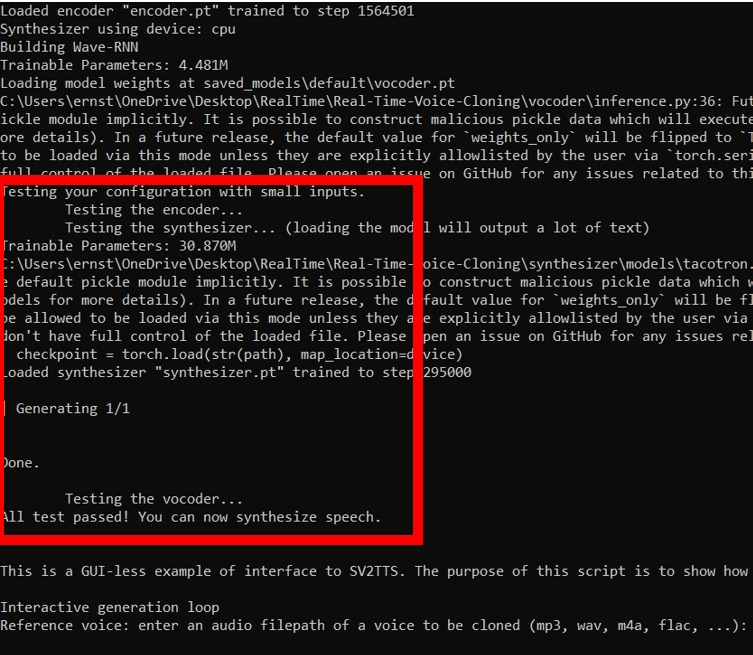
\includegraphics[width=1.0\textwidth]{Bilder/ToolboxTest}
    \centering
    \caption{Encoder, Vocoder und Synthesizer Test}
    \label{fig:KomponentenTest}
\end{figure}
Waren die Tests erfolgreich, kann das Skript demo\_toolbox.py ausgeführt werden, um die Toolbox zu öffnen.
\begin{figure}[H]
    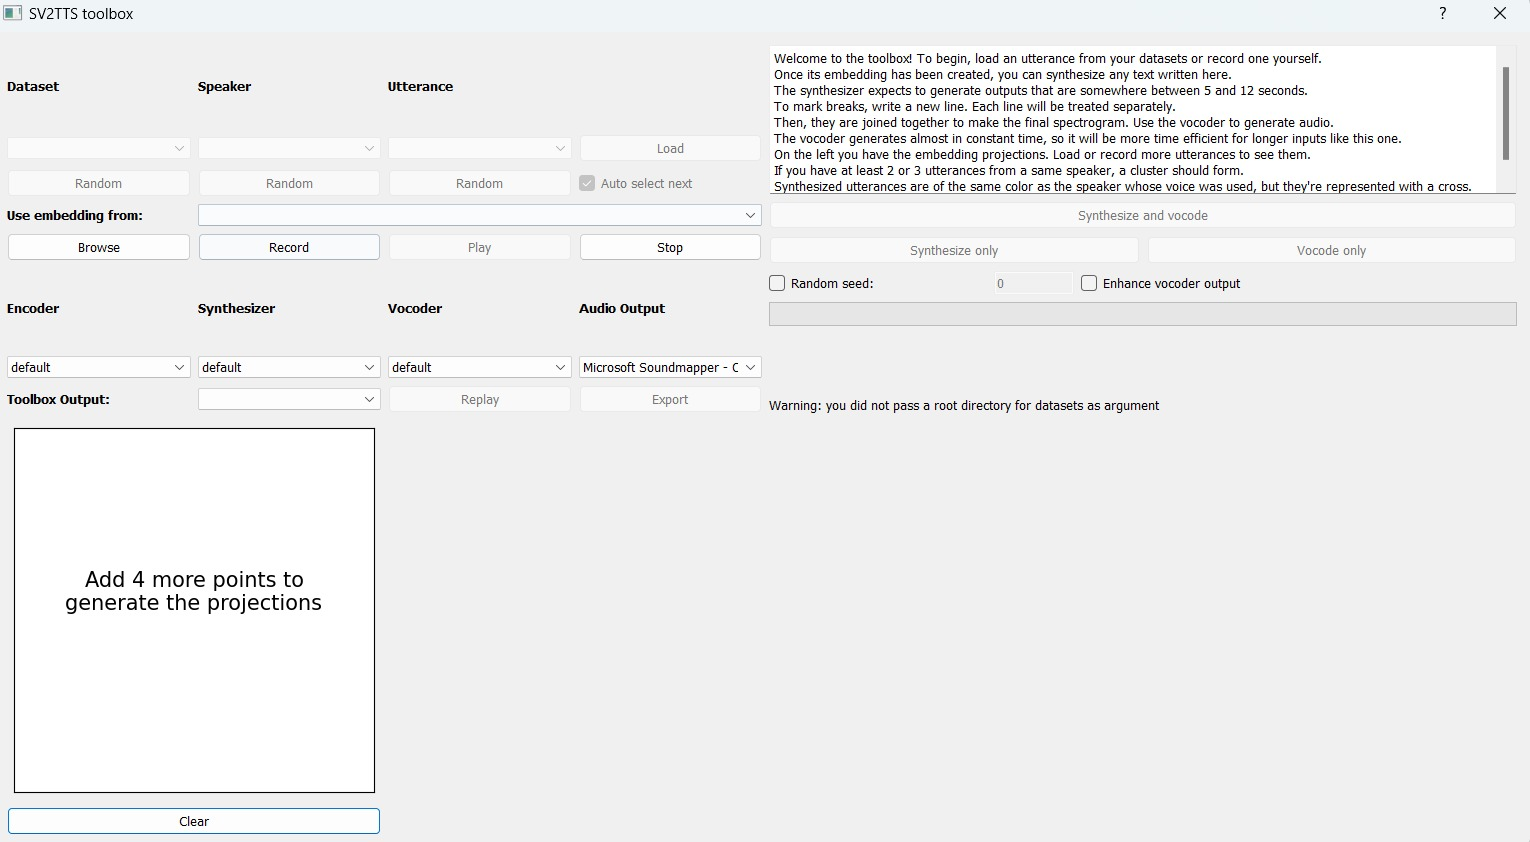
\includegraphics[width=1.0\textwidth]{Bilder/AudioToolbox1}
    \centering
    \caption{Real-Time Voice Cloning Toolbox}
    \label{fig:RTVCloningToolbox}
\end{figure}
\subsection{Extraktion}
Angekommen in der Toolbox, kann entweder eine bereits vorhandene Audiodatei eingegeben werden oder eine Echtzeit Aufnahme aufnehmen, um so das Trainingsmaterial der Toolbox bereitzustellen. Nachdem auswählen des Trainingsmaterial, kann die Stimme Sythetisiert und Vocoded werden. Zuerst wird ein Text eingegeben, was die geklonte Stimme wieder geben soll. Die Toolbox erstellt dann ein Mel Spektrogramm von dem Trainingmaterial und lässt dieses durch den Synthesizer durchlaufen, um an eine Audioausgabe zu gelangen. Nach einer kurzen Wartezeit wurde die Stimme geklont.
\begin{figure}[H]
    \includegraphics[width=1.0\textwidth]{Bilder/AudioToolbox2}
    \centering
    \caption{Real-Time Voice Cloning Toolbox nach Erzeugung der geklonten Stimme}
    \label{fig:RTVCloningToolboxDurchfuehrung}
\end{figure}